
Die in der \menu{*.bib} Datei erfassten Informationen zu der Quelle sind im Literatur- / Quellenverzeichnis aufgeführt.

\begin{figure}[h!]
\centering
  % 
\includegraphics[width=0.75\textwidth]{./Bilder/QuellenVerzeichnis.png}        % Bild ohne Rahmen
  \fbox{
\includegraphics[width=0.75\textwidth]{./Bilder/QuellenVerzeichnis.png}}   % Bild mit Rahmen
  \caption{Auflistung der Quellen im Literatur- / Quellenverzeichnis}
  \label{fig:QuellenVerzeichnis}
\end{figure} 

Erstellt wird das Literatur- / Quellenverzeichnis mit folgendem Befehl:

\begin{figure}[h!]
\centering
  % 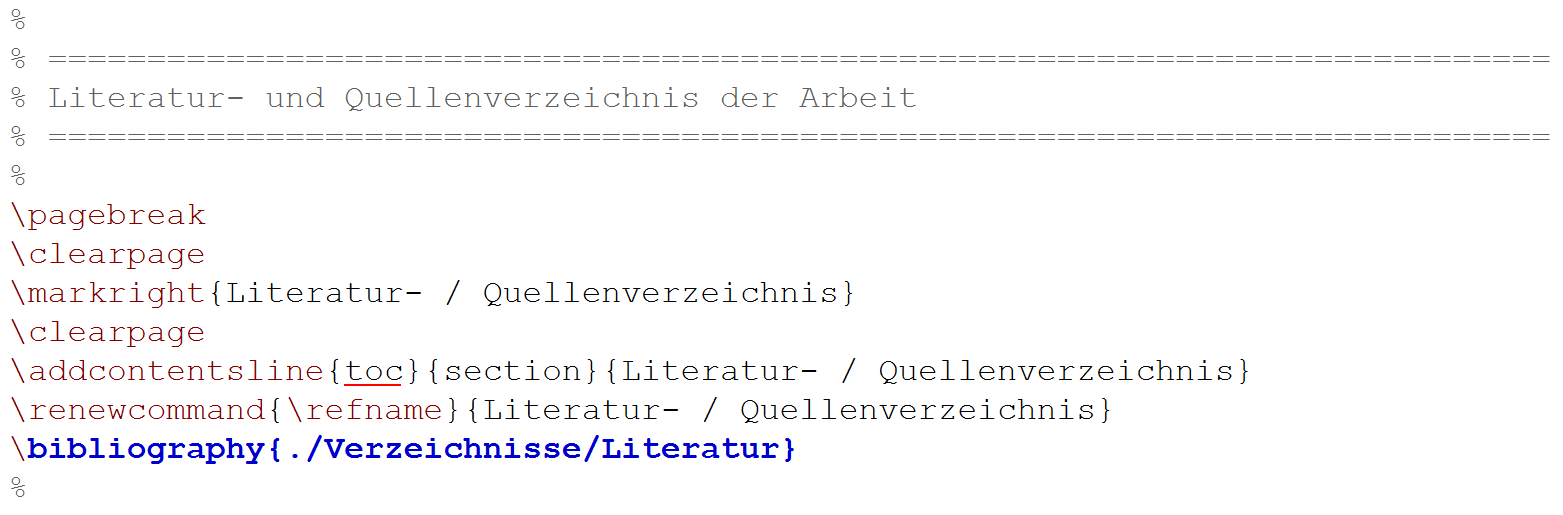
\includegraphics[width=0.75\textwidth]{./Bilder/QuellenVerzeichnisErstellen.png}        % Bild ohne Rahmen
  \fbox{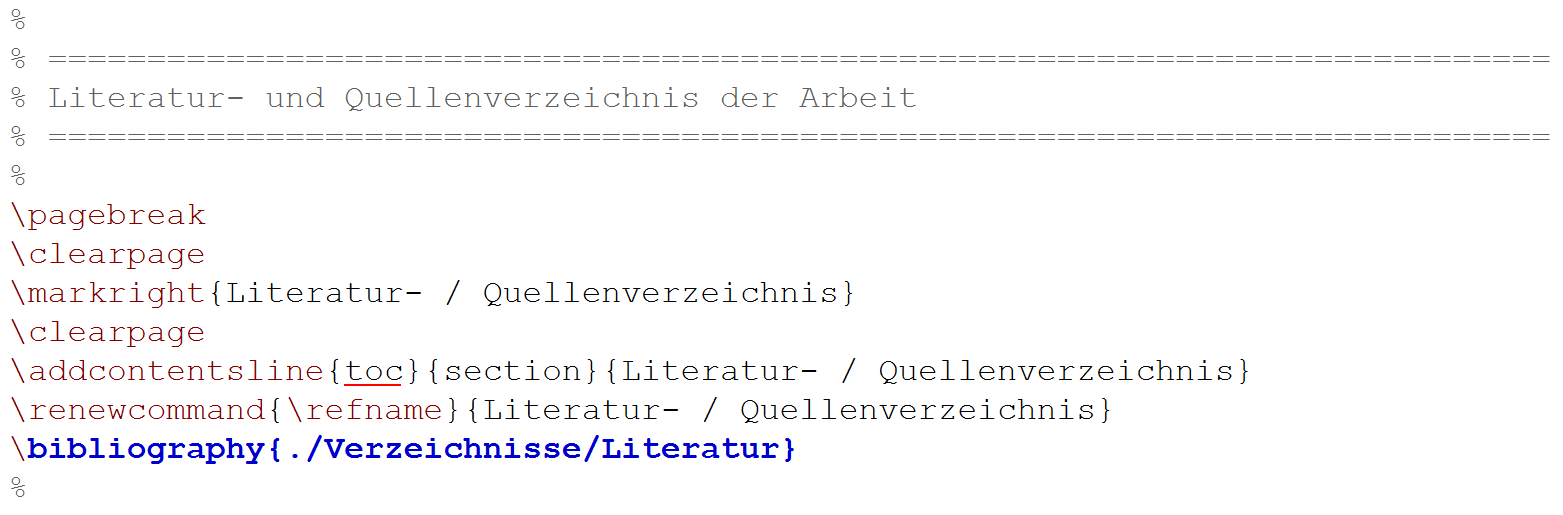
\includegraphics[width=0.75\textwidth]{./Bilder/QuellenVerzeichnisErstellen.png}}   % Bild mit Rahmen
  \caption{Erstellen des Literatur- / Quellenverzeichnis}
  \label{fig:QuellenVerzeichnisErstellen}
\end{figure} 
